\chapter{Systembeskrivelse}

Goofy Candygun 3000 er et underholdningssystem, som kan styres efter brugerønsker. Slikkanonen fungerer ved, at en bruger starter spillet på brugergrænsefladen på devkittet, derefter er spillet i gang. For at ændre sigteretningen for kanonen anvendes en Wii-nunchuck. Wii-nunchuck sender analogstikkets koordinater, via I2C kommunikation, til PSoC2. PSoC2 tolker dette data og sender kommandoen til PSoC0. PSoC0 videresender denne kommando til PSoC1. PSoC1 tolker denne kommando og udsender et PWM signal, som bevæger motorene efter den sendte kommando. Når der affyres et projektil sendes data om et knap tryk på Wii-nunchuck fra PSoC2 til PSoC1 via PSoC0. På figur \ref{ref:overordnetstruktur} ses den overordnede struktur af systemet. 

\begin{figure}[h]
	\centering
	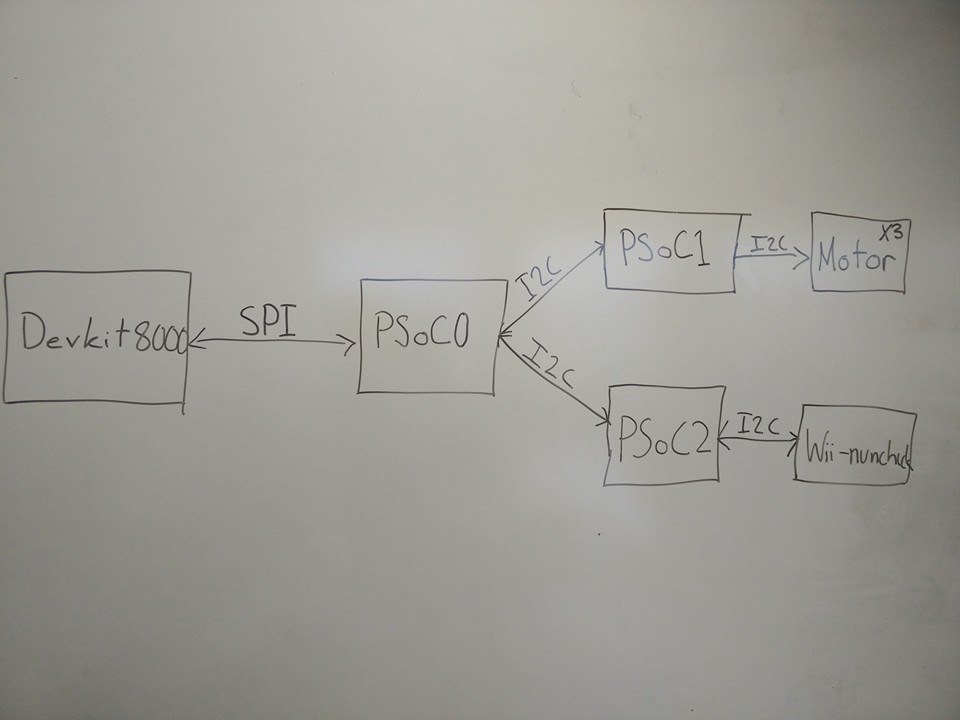
\includegraphics[width=\textwidth]{Systembeskrivelse/images/overordnetstruktur}
	\caption{Illustation af Goofy Candy 3000 overordnet struktur}
	\label{ref:overordnetstruktur}
\end{figure}



HUSK BILLEDE OG FORKLARING AF ENDELIG UDSEENDE.